\documentclass[12pt,a4paper]{article}

\usepackage[margin=1in]{geometry}
\usepackage{setspace}
\usepackage{graphicx}
\usepackage{amsmath}
\usepackage{hyperref}
\hypersetup{hidelinks}
\usepackage{pgfgantt}
\usepackage[nonumberlist,acronym,nomain]{glossaries}
\loadglsentries{acronyms.tex}

\usepackage{algorithm}
\usepackage{algpseudocode}



\usepackage{xcolor}
\usepackage{lmodern}
\usepackage[T1]{fontenc}
\usepackage{tikz}
\usepackage{subcaption}
\usetikzlibrary{positioning,arrows.meta}
%------------------------------------------------
% Custom colors
%------------------------------------------------
\definecolor{timelineblue}{RGB}{27,82,158}
\definecolor{timelinegreen}{RGB}{91,153,51}
\definecolor{timelinepurple}{RGB}{124,89,185}

\definecolor{phaseblue}{RGB}{232,241,252}
\definecolor{phasegreen}{RGB}{238,246,231}
\definecolor{phasepurple}{RGB}{243,237,250}

\definecolor{headerblue}{RGB}{8,35,78}
\definecolor{gridgray}{RGB}{205,205,205}
\usetikzlibrary{
    positioning,
    arrows.meta,
    fit,
    calc,
    shapes.geometric
}


\begin{document}

\begin{titlepage}
    \centering
    
    {\Large Aalen University of Applied Science \par}
    \vspace{0.5cm}
    {\large Faculty of Electronics and Computer Science \par}
      \vspace{1cm}
    {\Large PhD Research Proposal \par}
    \vspace{6cm}
    
    {\Huge \textbf{Adaptive MAC Scheduling and Resource Allocation for DECT-2020 NR Industrial IoT Networks} \par}
    
    \vspace{1.5cm}
    
    
    
    \vspace{6cm}
    
    \begin{flushleft}
    \textbf{Submitted by:} Ashuqullah Alizai \\
    \textbf{Email:} ashuqullah.alizai@hs-aalen.de\\
    \textbf{Supervisor:} Prof. Dr. Stephan Ludwig \\
    \textbf{Department:} Communications  \\
    \end{flushleft}
    
    \vfill
    
    {\large \today \par}
    
\end{titlepage}



\begin{abstract}

\begin{abstract}

\gls{nr} is an \gls{etsi}-standardized wireless access technology designed for \gls{iiot} applications, offering flexible deployment, operation in dedicated spectrum bands, and support for private wireless networks. Recent studies have demonstrated its capability to provide reliable and low-latency communication in industrial environments. However, existing research primarily focuses on protocol evaluation and performance characterization, while application-oriented \gls{mac}-layer mechanisms remain largely unexplored.

Industrial applications exhibit diverse communication requirements, ranging from deterministic control traffic with stringent latency and jitter constraints to energy-constrained sensing applications requiring long device sleep times. Efficient support for these requirements depends on appropriate scheduling and resource allocation mechanisms that also consider practical implementation constraints, including \gls{tdd} operation, \gls{rx}-to-\gls{tx} turnaround time, and multi-channel communication.

This research investigates adaptive \gls{mac}-layer scheduling and resource allocation mechanisms for \gls{nr} that are tailored to different industrial application requirements. Rather than relying on a single generic scheduler, the proposed framework enables different scheduling and resource allocation strategies for deterministic industrial communication, highly reliable data transmission, and energy-efficient operation.

The proposed methodology combines protocol design, analytical modeling, implementation, and measurement-based validation using a real \gls{nr} hardware platform. The expected outcome is a practical application-oriented \gls{mac} framework that improves latency, reliability, scalability, and energy efficiency while providing design guidelines for future \gls{nr} industrial deployments.

\end{abstract}
\end{abstract}
\section{Introduction}

Industrial wireless communication systems are increasingly used to support monitoring, control, automation, and coordination tasks in modern production environments. Applications such as factory automation, closed-loop control, condition monitoring, mobile robotics, and battery-powered sensing impose substantially different requirements regarding latency, jitter, reliability, scalability, and energy consumption \cite{willigWirelessTechnologyIndustrial2005,vitturiIndustrialWirelessNetworks2013,wollschlaegerFutureIndustrialCommunication2017a}. Consequently, a single wireless technology or network configuration may not satisfy all industrial use cases. Heterogeneous communication architectures combining different local and cellular technologies have therefore emerged as an important enabler of Industry~4.0 and smart manufacturing \cite{alizaiHeterogeneousCommunicationNetworks2023a,karrenbauerFutureIndustrialNetworking2019a,aschenbrennerFlexiCell5GLocationbased2022a}.

\gls{nr} is an \gls{etsi}-standardized radio access technology developed within the IMT-2020 framework for local-area and massive-machine-type communication. The technology supports autonomous and decentralized network formation without requiring the conventional base-station and core-network architecture of cellular systems \cite{kovalchukovDECT2020NewRadio2022,perez-guiraoDECTNRUnveiling2022}. It is intended for applications such as industrial monitoring, building automation, smart metering, professional audio, critical-infrastructure communication, and other \gls{iot}/\gls{iiot} scenarios \cite{durreDECT2020NRProfessional2024,poetsProfessionalNetworkedAudio2025,biswasReliableLowLatencyCommunications2024}. Its operation is defined for dedicated DECT spectrum and additional frequency bands subject to the applicable regional regulatory framework \cite{etsi_tr103943}.

The DECT-2020 NR protocol architecture is defined in the ETSI TS~103~636 series. The \gls{phy} layer specifies radio transmission and reception procedures, while the \gls{mac} layer defines mechanisms for channel access, beaconing, association, random access, resource allocation, scheduled transmission, and group communication \cite{etsi_ts103636_1,etsi_ts103636_3,etsi_ts103636_4}. Radio devices may operate as \glspl{ft}, \glspl{pt}, or simultaneously in both roles, enabling point-to-point, point-to-multipoint, and multi-hop network topologies. Although the standard specifies the messages, timing relationships, and resource structures required for interoperable operation, the selection and implementation of application-specific scheduling policies remain an open design task.

In this research, \textit{resource allocation} denotes the assignment of radio resources, including frequency channels, subslots, slots, and transmission opportunities, to communicating devices. \textit{\gls{mac} scheduling} denotes the policy used to determine how and when the allocated resources are used by individual devices or groups of devices. Random access controls contention-based network entry and unscheduled transmission opportunities, whereas group assignment allows multiple devices with related communication requirements to be coordinated through common resource configurations. These mechanisms jointly determine whether a DECT-2020 NR deployment can meet application-specific requirements for latency, jitter, reliability, scalability, and energy consumption.

Existing studies have demonstrated that DECT-2020 NR can satisfy important IMT-2020 performance requirements and support low-latency and massive-device communication under selected configurations \cite{dhanwaniAssessmentCandidateTechnology2020,pennerURLLCPerformanceEvaluation2021,smidaETSIDECT2020Component2023}. Experimental investigations have further evaluated its physical-layer performance, communication range, energy consumption, and suitability for industrial and professional-audio environments \cite{wassmannPerformanceDECT2020NR2024,haqueDECT2020NRLink2025,grafWhatExpectWhen2026,durreDECT2020NRProfessional2024}. However, much of the current literature concentrates on feasibility assessment, link- and system-level performance, or isolated protocol enhancements rather than on the systematic design of application-oriented scheduling and resource-allocation mechanisms.

Industrial applications require different MAC-layer behavior. First, deterministic control communication, including periodic sensor--actuator exchange and industrial control loops, requires bounded communication latency, low jitter, and predictable cycle times. These requirements differ from conventional wireless scheduling objectives that primarily maximize throughput or fairness \cite{vitturiIndustrialWirelessNetworks2013,popovskiWirelessAccessUltraReliable2018,bennisUltrareliableLowLatencyWireless2018a}. Second, reliability-critical communication, such as alarms, protection messages, and infrastructure monitoring, requires highly dependable packet delivery and may benefit from resource redundancy, channel diversity, or coordinated multi-channel transmission \cite{biswasReliableLowLatencyCommunications2024,glazkovImprovingNearURLLCServices2025,ahmadMACLayerProtocolUltraReliable2025}. Third, battery-powered sensing applications require long sleep intervals and carefully configured transmission and reception opportunities in order to reduce energy consumption while respecting application-specific latency constraints \cite{nihtilaEnergyConsumptionDECT20202022,nihtilaEnergySavingRouter2022,grafWhatExpectWhen2026}.

In this proposal, the term \textit{adaptive} does not imply machine-learning-based control or continuous autonomous optimization during operation. Instead, it denotes the capability to configure and select different DECT-2020 NR MAC strategies according to the requirements of a particular application or deployment scenario. A deterministic industrial-control application may employ reserved and group-based transmission resources; a reliability-critical application may use redundant or multi-channel assignments; and an energy-constrained sensing application may use sparse transmission opportunities and application-specific receive windows. Adaptation therefore refers to the systematic mapping of application requirements to suitable scheduling, resource-allocation, random-access, and group-assignment configurations.

Practical implementation constraints must also be considered. DECT-2020 NR communication performance is influenced not only by the abstract resource structure defined by the standard but also by \gls{tdd} timing, processing delays, schedule-distribution overhead, and \gls{rx}-to-\gls{tx} turnaround behavior. Preliminary measurements on the available DECT-2020 NR hardware platform indicate that such implementation effects can contribute substantially to end-to-end latency, particularly for short-packet and request--response communication. Scheduler design must therefore account for both application requirements and the timing limitations of the actual platform.

Accordingly, this research aims to design, implement, and experimentally validate adaptive \gls{mac}-layer scheduling and resource-allocation mechanisms for \gls{nr}. The work focuses on three representative industrial communication classes: deterministic control communication, reliability-oriented communication, and energy-efficient sensing. For these application classes, suitable mechanisms for scheduled access, resource assignment, random access, group formation, and multi-channel operation will be developed and evaluated through analytical modeling, simulation, protocol implementation, and real-hardware experimentation. The overall objective is to establish an application-oriented MAC framework and practical design guidelines for improving latency, jitter, reliability, scalability, and energy efficiency in industrial DECT-2020 NR deployments.



\section{Background and Related Work}
\subsection{Industrial Wireless Communication Requirements}

Industrial automation and \gls{iiot} applications require wireless communication systems capable of supporting heterogeneous and, in some cases, conflicting performance requirements. As illustrated in Figure~\ref{fig:industrial_requirements}, modern industrial environments encompass a wide range of applications, including industrial control, condition monitoring, safety systems, logistics, and multimedia services. Although these applications operate within the same communication infrastructure, their communication requirements differ significantly in terms of latency, reliability, scalability, energy consumption, and \gls{qos} \cite{willigWirelessTechnologyIndustrial2005,vitturiIndustrialWirelessNetworks2013,wollschlaegerFutureIndustrialCommunication2017a,boyesIndustrialInternetThings2018,sisinniIndustrialInternetThings2018}.

\begin{figure}[htbp]
    \centering
    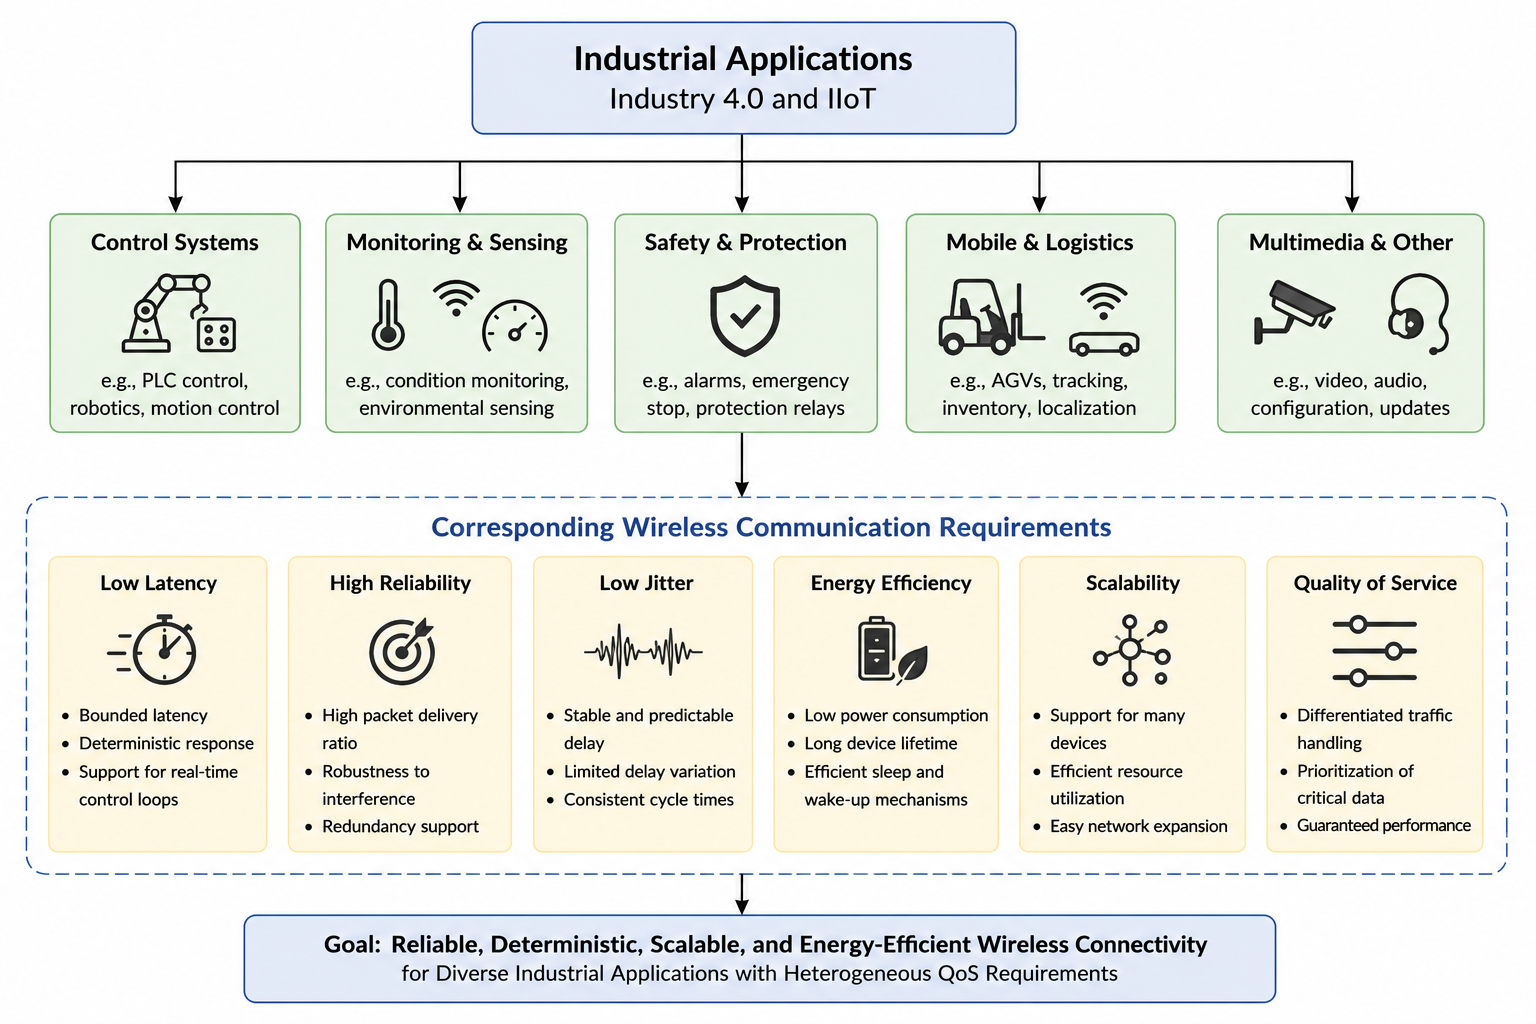
\includegraphics[width=\textwidth]{figures/IndustrialReq.png}
    \caption{Relationship between representative industrial applications and their corresponding wireless communication requirements.}
    \label{fig:industrial_requirements}
\end{figure}

Industrial control systems, such as \glspl{plc}, robotic manipulators, and motion-control applications, typically require deterministic communication with bounded latency, low jitter, predictable cycle times, and extremely high packet-delivery reliability. In contrast, monitoring and sensing applications generally tolerate longer communication delays but prioritize low energy consumption, extended device lifetime, and support for a large number of battery-powered devices. Safety and protection systems require highly dependable and timely message delivery, whereas mobile and logistics applications, including autonomous guided vehicles (AGVs) and asset tracking, demand reliable connectivity under mobility and varying channel conditions. Multimedia and maintenance-related applications, such as video surveillance, remote diagnostics, and software updates, primarily emphasize throughput and efficient resource utilization rather than stringent latency requirements \cite{willigWirelessTechnologyIndustrial2005,vitturiIndustrialWirelessNetworks2013,wollschlaegerFutureIndustrialCommunication2017a,sisinniIndustrialInternetThings2018}.

The diversity of industrial communication requirements has motivated the deployment of heterogeneous networking infrastructures that combine multiple wired and wireless technologies according to application, coverage, and performance requirements \cite{alizaiHeterogeneousCommunicationNetworks2023a,karrenbauerFutureIndustrialNetworking2019a,aschenbrennerFlexiCell5GLocationbased2022a}. Although such architectures provide considerable flexibility, they also increase system complexity, deployment effort, and network management overhead. Consequently, emerging wireless technologies designed for private, locally managed, and independently operated networks have attracted increasing attention because they offer configurable communication behavior without relying on conventional public cellular infrastructure.

\gls{nr} represents one such technology. Its decentralized operation, flexible network topology, and support for both scheduled and contention-based communication make it well suited to industrial environments with heterogeneous traffic characteristics and diverse application requirements. However, the suitability of \gls{nr} for industrial applications depends not only on the capabilities defined by the standard but also on how efficiently its \gls{mac}-layer mechanisms allocate radio resources, schedule transmissions, and satisfy diverse \gls{qos} requirements under varying network conditions \cite{etsi_ts103636_1,etsi_ts103636_4,perez-guiraoDECTNRUnveiling2022,kovalchukovDECT2020NewRadio2022,poetsDECTNRNew2024}.

Consequently, industrial wireless communication systems must provide reliable, scalable, and energy-efficient connectivity while simultaneously accommodating heterogeneous traffic with diverse quality-of-service requirements \cite{willigWirelessTechnologyIndustrial2005,vitturiIndustrialWirelessNetworks2013,wollschlaegerFutureIndustrialCommunication2017a}. Achieving these objectives depends not only on the capabilities of the underlying physical layer but also on efficient medium access and resource management. This motivates the investigation of \gls{nr}, whose flexible \gls{mac}-layer architecture provides the foundation for developing adaptive scheduling and resource-allocation mechanisms suitable for next-generation industrial wireless networks.
% =====================================================


\subsection{DECT-2020 NR Architecture and MAC Operation}
\label{subsec:dect-architecture-mac}
\gls{nr} is a radio-interface technology standardized by \gls{etsi} and included in the IMT-2020 family. It was developed to support local wireless communication, massive machine-type connectivity, and low-latency industrial applications through autonomous and decentralized network formation \cite{kovalchukovDECT2020NewRadio2022,dhanwaniAssessmentCandidateTechnology2020}. Unlike conventional cellular systems, DECT-2020 NR does not depend on a permanently deployed base station and core-network infrastructure. Instead, devices establish local and private wireless networks in which communication is coordinated autonomously according to their assigned roles and the selected network topology.

The protocol architecture is specified in the ETSI TS~103~636 series. Part~1 defines the overall system architecture, whereas the subsequent parts specify the \gls{phy} and \gls{mac} layers together with the associated radio procedures \cite{etsi_ts103636_1,etsi_ts103636_2,etsi_ts103636_3,etsi_ts103636_4}. As illustrated in Figure~\ref{fig:dectnr_architecture_mac}, the protocol stack consists of the application layer, the \gls{mac} layer, the \gls{phy} layer, and the RF front-end. The application layer hosts industrial services and application-specific communication functions. The \gls{phy} layer defines waveform generation, modulation, coding, numerology, channel structure, and radio transmission procedures, while the \gls{mac} layer coordinates higher-level communication functions including beacon transmission, network discovery, association, random access, resource scheduling, feedback, and group communication.

A DECT-2020 NR device may operate as a \gls{ft}, a \gls{pt}, or in both roles. The \gls{ft} acts as the local network coordinator by periodically transmitting synchronization beacons, managing communication resources, and distributing scheduling and control information to the associated \glspl{pt}. The \glspl{pt} use the allocated resources to exchange application data and return acknowledgement or status information to the \gls{ft}. Devices supporting both roles may additionally relay traffic and extend network coverage through multi-hop forwarding, enabling star, tree, and mesh-like communication topologies. In this research, however, the focus is restricted to controlled star-topology deployments, where a single \gls{ft} coordinates multiple \glspl{pt} in a reproducible industrial environment.

Figure~\ref{fig:dectnr_architecture_mac} also summarizes the principal DECT-2020 NR communication cycle. Communication begins with periodic beacon transmission by the \gls{ft}, enabling nearby devices to synchronize with the network and obtain control information. Portable terminals subsequently perform network discovery by scanning available radio channels and identifying suitable DECT-2020 NR networks. During the association phase, a \gls{pt} requests network access and receives the addressing and configuration information required for communication.

Once association has been completed, the \gls{ft} allocates the available time-frequency resources and distributes the corresponding scheduling information. The \glspl{pt} then exchange uplink and downlink data using the assigned communication resources, either through scheduled or contention-based access depending on the selected communication mode. After each transmission cycle, acknowledgement and feedback messages provide information about successful reception, channel conditions, and transmission status. Based on this feedback and current traffic demands, the \gls{ft} updates the scheduling decisions and resource allocations before broadcasting the next beacon, thereby initiating a new communication cycle.

Although DECT-2020 NR specifies the protocol procedures and available communication mechanisms, it deliberately leaves the scheduling and resource-allocation strategy implementation-dependent. Consequently, system designers must determine how transmission opportunities are assigned, how communication resources are shared among devices, and how scheduling decisions are adapted to heterogeneous industrial traffic requirements. Different implementations may therefore exhibit substantially different latency, reliability, scalability, fairness, and energy-efficiency characteristics despite complying with the same standard. This implementation flexibility forms the foundation of the proposed research on adaptive MAC scheduling and resource allocation for industrial DECT-2020 NR networks.
\begin{figure}[htbp]
    \centering
    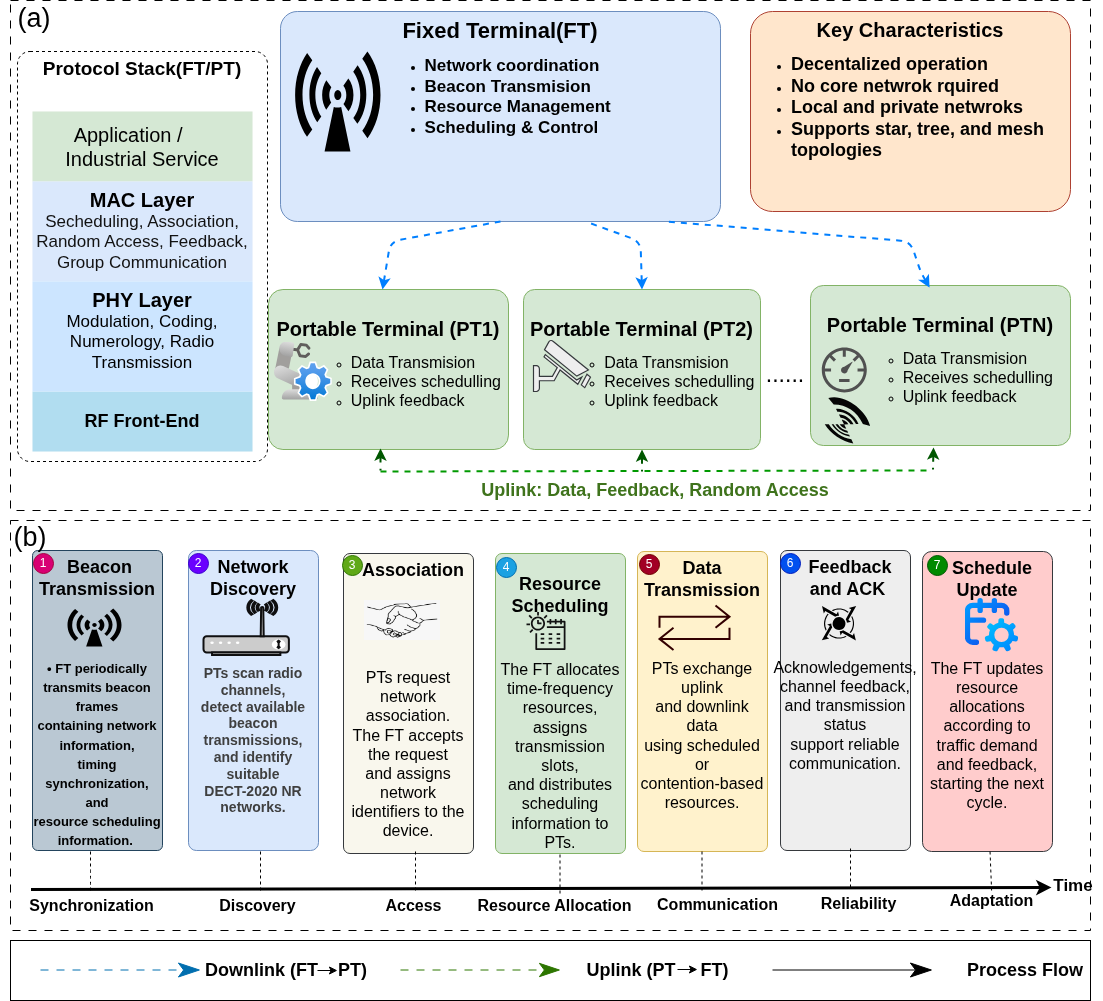
\includegraphics[width=\textwidth]{figures/archetictur.png}
    \caption{Overview of the DECT-2020 NR architecture and MAC operation. The upper part illustrates the protocol architecture, Fixed Terminal, Portable Terminals, and the principal uplink and downlink communication paths. The lower part summarizes the MAC communication cycle, including beacon transmission, network discovery, association, resource scheduling, data transmission, feedback, and schedule update.}
    \label{fig:dectnr_architecture_mac}
\end{figure}


% =====================================================

\subsection{Scheduling and Resource Allocation in DECT-2020 NR Wireless Networks}
\label{subsec:scheduling}

Scheduling and resource allocation are fundamental functions of the \gls{mac} layer that determine how multiple devices share limited wireless communication resources. Their primary objective is to coordinate channel access while satisfying application-specific performance requirements such as latency, reliability, throughput, fairness, and energy efficiency. Unlike wired communication, wireless scheduling must continuously account for time-varying channel conditions, interference, half-duplex operation, transmission errors, and dynamic network topology, making resource allocation significantly more challenging \cite{luFairSchedulingWireless1999a,fattahOverviewSchedulingAlgorithms2002a}.

Traditional wireless scheduling algorithms have largely focused on maximizing system throughput, improving spectral efficiency, and achieving fairness among competing users. Numerous scheduling strategies have been proposed for cellular and wireless networks, including round-robin, proportional-fair, maximum-rate, earliest-deadline-first, and priority-based schedulers. These approaches are generally designed to balance throughput, fairness, packet delay, jitter, and channel utilization while adapting to changing radio conditions \cite{andrewsProvidingQualityService2001,fattahOverviewSchedulingAlgorithms2002a}. Although these objectives remain important, they do not fully address the communication requirements of industrial wireless systems.

Industrial applications impose substantially different requirements depending on the communication scenario. Periodic control traffic requires deterministic transmission opportunities with bounded latency and minimal jitter to ensure predictable control-loop execution. Reliability-critical applications prioritize successful packet delivery and rapid recovery from transmission failures, whereas battery-powered sensing devices require communication schedules that maximize sleep intervals and minimize unnecessary radio activity. Consequently, resource-allocation decisions must be tailored to the specific traffic characteristics rather than relying solely on throughput-oriented optimization.

Within DECT-2020 NR, scheduling is performed by the \gls{ft}, which coordinates communication resources for the associated \glspl{pt}. As illustrated in Figure~\ref{fig:dectnr_architecture_mac}, the scheduling process follows network discovery and association, after which the \gls{ft} assigns the available time-frequency resources and distributes scheduling information through beacon and control signaling. During subsequent communication cycles, \glspl{pt} exchange uplink and downlink data using the allocated resources and provide feedback that enables the \gls{ft} to adapt future scheduling decisions according to current network conditions and application requirements.

The DECT-2020 NR standard defines the available resource structures, signaling procedures, and communication mechanisms but intentionally does not prescribe a fixed scheduling strategy. Implementers are therefore responsible for determining how transmission opportunities are allocated, how resources are shared among multiple devices, how random-access resources are configured, and how scheduling decisions are adapted over time. As a result, different DECT-2020 NR implementations may exhibit significantly different latency, reliability, fairness, scalability, and energy-consumption characteristics, despite fully complying with the same protocol specification.

Although numerous optimization and resource-allocation techniques have been proposed for LTE and 5G systems, including priority-aware, delay-aware, and optimization-based schedulers \cite{andrewsProvidingQualityService2001,liuEfficientResourceAllocation2024,bahetiPriorityawareRadioResource2026nr1}, these approaches generally assume centralized cellular architectures, different frame structures, and different control procedures. Consequently, their direct application to DECT-2020 NR remains limited. This research therefore investigates application-aware adaptive MAC scheduling and resource-allocation mechanisms specifically designed for industrial DECT-2020 NR networks, where scheduling decisions are tailored to the heterogeneous requirements of deterministic control, reliability-oriented communication, and energy-efficient sensing applications.
% =====================================================

\subsection{Random Access and Group-Based Communication}
\label{subsec:random_access}

Random access is an essential mechanism in wireless networks that enables devices to transmit when dedicated communication resources have not yet been assigned or when sporadic data must be delivered outside an existing schedule. Its performance is strongly influenced by the number of contending devices, contention-window configuration, collision probability, retransmission strategy, and access-response timing. As network density increases, contention-based access may result in repeated collisions, increased access delay, reduced reliability, and higher energy consumption because devices repeatedly attempt channel access or remain active while waiting for network responses \cite{andrewsProvidingQualityService2001,fattahOverviewSchedulingAlgorithms2002a}.

Within DECT-2020 NR, random access supports several fundamental communication procedures, including initial network association and contention-based data transmission. The ETSI specification defines the signaling messages, timing relationships, and protocol procedures required for random access, while leaving the selection of operational parameters to the system implementation \cite{etsi_ts103636_4}. Consequently, network performance depends not only on the standardized protocol but also on how random-access opportunities are configured for a particular deployment. Recent work has demonstrated that random-access delay in DECT-2020 NR can be reduced by estimating the number of active devices and dynamically adapting the access procedure, illustrating the importance of deployment-aware parameter configuration \cite{gaidamakaOptimizingDelaysRandom2025}.

For industrial wireless applications, random access is particularly important for event-driven communication, including alarms, fault notifications, and sporadic sensor updates, where transmission requests occur unpredictably and cannot always be reserved in advance \cite{willigWirelessTechnologyIndustrial2005,vitturiIndustrialWirelessNetworks2013,wollschlaegerFutureIndustrialCommunication2017a}. Since these transmissions cannot be scheduled deterministically beforehand, reserving dedicated communication resources for every possible event would lead to inefficient resource utilization and reduced spectrum efficiency \cite{andrewsProvidingQualityService2001}. Conversely, relying exclusively on contention-based access under high network load may result in increased collision probability, longer access delays, and degraded reliability for time-critical applications \cite{fattahOverviewSchedulingAlgorithms2002a,gaidamakaOptimizingDelaysRandom2025}. Consequently, an industrial \gls{mac} design should combine deterministic scheduled resources for periodic traffic with carefully configured random-access opportunities for sporadic and event-driven communication, thereby balancing responsiveness, reliability, and resource efficiency.

Group-based communication provides an additional mechanism for improving scheduling efficiency in networks containing large numbers of devices with similar communication characteristics. Devices may be grouped according to application cycle, traffic periodicity, latency requirements, reliability constraints, or energy-consumption objectives. Rather than scheduling each device independently, the coordinator may allocate common communication resources or shared transmission opportunities to an entire group. Such coordination reduces scheduling overhead, simplifies schedule dissemination, and can improve resource utilization, particularly in industrial monitoring and control systems where many devices exhibit similar communication patterns \cite{etsi_ts103636_4}.

Despite its potential benefits, group-based communication introduces several scheduling challenges. Devices assigned to the same group must remain sufficiently synchronized to ensure coordinated resource usage, while heterogeneous communication requirements within a group may increase waiting time, reduce resource utilization, or compromise deterministic performance \cite{willigWirelessTechnologyIndustrial2005,vitturiIndustrialWirelessNetworks2013}. Consequently, effective group formation should consider application timing, traffic characteristics, device capabilities, latency requirements, and the availability of communication resources to achieve an appropriate balance between efficiency and quality of service \cite{andrewsProvidingQualityService2001,fattahOverviewSchedulingAlgorithms2002a}. These trade-offs become increasingly significant as the number of connected devices grows and multiple heterogeneous industrial applications coexist within the same wireless network \cite{wollschlaegerFutureIndustrialCommunication2017a}.

Although DECT-2020 NR provides standardized signaling procedures and resource-allocation mechanisms that support both contention-based access and group-oriented communication \cite{etsi_ts103636_4}, our systematic review of the current DECT-2020 NR literature indicates that existing studies have primarily concentrated on protocol architecture, implementation, performance evaluation, and isolated optimization problems, while adaptive MAC scheduling for heterogeneous industrial applications has received comparatively limited attention \cite{gaidamakaOptimizingDelaysRandom2025,kovalchukovDECT2020NewRadio2022}. In particular, few studies jointly consider application requirements, random-access configuration, device grouping, schedule dissemination, and practical hardware timing within a unified scheduling framework. Addressing these challenges forms one of the central objectives of the proposed research.

% =====================================================

\subsection{DECT-2020 NR Performance Evaluation and MAC Enhancements}
\label{subsec:performance_mac_enhancements}

Early DECT-2020 NR research primarily investigated whether the technology could satisfy the performance requirements associated with IMT-2020 and massive machine-type communication. System-level and link-level studies evaluated aspects such as latency, reliability, connection density, coverage, and support for large device populations
\cite{dhanwaniAssessmentCandidateTechnology2020,
anttonenEnablingMassiveMachine2021a,
pennerURLLCPerformanceEvaluation2021,
smidaETSIDECT2020Component2023}.
These studies established the general technical feasibility of DECT-2020 NR, but their conclusions were largely based on analytical models, simulations, or predefined system configurations rather than complete hardware-based implementations.

More recent work has shifted toward experimental evaluation using hardware prototypes and real radio environments. These studies have examined physical-layer performance, communication range, scalability, energy consumption, implementation behavior, and the feasibility of selected application scenarios
\cite{wassmannPerformanceDECT2020NR2024,
haqueDECT2020NRLink2025,
bandaraExperimentalValidationAnalysis2025,
grafWhatExpectWhen2026}.
Experimental investigations in factory-automation environments have also evaluated DECT-2020 NR under industrial propagation conditions
\cite{llagunoPhysicalLayerPerformance2024}.
Such studies provide important evidence regarding achievable communication performance and practical deployment limitations. However, they generally evaluate the technology using fixed configurations and do not develop comprehensive application-aware scheduling frameworks.

Several publications have proposed specific MAC-layer, routing, or reliability enhancements. Ahmad et al. introduced a MAC protocol intended to reduce outage probability in DECT-2020 NR networks
\cite{ahmadMACProtocolReducing2024},
while subsequent work investigated MAC-layer mechanisms for ultra-reliable multi-hop \gls{iiot} communication
\cite{ahmadMACLayerProtocolUltraReliable2025}.
Other studies have explored near-\gls{urllc} operation in multi-hop networks, reliability-oriented resource prioritization, and assisted communication mechanisms
\cite{glazkovImprovingNearURLLCServices2025,
binasifIRSAssistedDECT2020NR2025}.
These contributions address important individual aspects of reliability, routing, or resource allocation. Nevertheless, they do not jointly consider deterministic scheduling, group-based coordination, energy-aware operation, random-access configuration, and implementation-specific timing constraints within a unified \gls{mac} framework.

Energy consumption has also received attention in the DECT-2020 NR literature. Nihtilä et al. analyzed device-level energy consumption and proposed energy-saving operation for routing devices
\cite{nihtilaEnergyConsumptionDECT20202022,
nihtilaEnergySavingRouter2022}.
Their results indicate that radio activity, device role, reception behavior, and routing responsibilities can significantly influence energy consumption. However, the systematic coordination of transmission schedules, reception windows, sleep intervals, and application latency constraints remains insufficiently addressed.

Research on professional audio and other latency-sensitive applications further demonstrates that DECT-2020 NR can support specialized communication services when protocol and resource configurations are carefully selected
\cite{durreDECT2020NRProfessional2024,
poetsProfessionalNetworkedAudio2025}.
These studies provide valuable application-specific insights, particularly concerning low-latency and synchronized communication. Nevertheless, their solutions are tailored to particular use cases and do not provide a general scheduling framework for heterogeneous industrial traffic comprising deterministic control, reliability-critical communication, sporadic events, and energy-efficient sensing.

Overall, the reviewed literature can be grouped into four broad categories: standardization and architectural studies, IMT-2020-oriented performance evaluations, experimental feasibility investigations, and individual MAC-layer, routing, or reliability enhancements. Despite this progress, a comprehensive and experimentally validated methodology for translating heterogeneous industrial application requirements into DECT-2020 NR scheduling and resource-allocation decisions remains missing. In particular, existing studies do not jointly address deterministic transmission timing, random-access configuration, group formation, multi-channel allocation, energy-aware reception scheduling, and practical hardware constraints. 
Despite this progress, a comprehensive and experimentally validated methodology
for translating heterogeneous industrial application requirements into
DECT-2020 NR scheduling and resource-allocation decisions remains missing.
Addressing this gap constitutes a central objective of the proposed research.
% =====================================================

\subsection{Research Gap}
\label{subsec:research_gap}

The existing DECT-2020 NR literature has established the feasibility of the technology, evaluated its performance under selected configurations, and proposed improvements to individual protocol mechanisms
\cite{dhanwaniAssessmentCandidateTechnology2020,
anttonenEnablingMassiveMachine2021a,
pennerURLLCPerformanceEvaluation2021,
wassmannPerformanceDECT2020NR2024,
ahmadMACProtocolReducing2024,
nihtilaEnergyConsumptionDECT20202022}.
However, these contributions do not yet provide a comprehensive, application-oriented \gls{mac} design methodology for heterogeneous industrial deployments.

The first research gap concerns deterministic industrial communication. Periodic control and sensor--actuator applications require bounded latency, low jitter, and predictable communication cycles. Existing DECT-2020 NR studies mainly evaluate average latency, reliability, or packet-delivery performance under predefined configurations
\cite{pennerURLLCPerformanceEvaluation2021,
smidaETSIDECT2020Component2023,
llagunoPhysicalLayerPerformance2024,
bandaraExperimentalValidationAnalysis2025}.
They provide limited guidance on how transmission resources should be assigned when application periods do not align directly with the DECT-2020 NR timing structure. In particular, the joint design of resource reservation, schedule repetition, schedule dissemination, and practical \gls{tdd} timing for minimizing cycle-to-cycle latency variation remains insufficiently investigated.

The second gap concerns reliability-oriented communication. Existing studies have proposed outage-reduction mechanisms, multi-hop reliability enhancements, and resource-prioritization approaches
\cite{ahmadMACProtocolReducing2024,
ahmadMACLayerProtocolUltraReliable2025,
glazkovImprovingNearURLLCServices2025,
binasifIRSAssistedDECT2020NR2025}.
Nevertheless, limited attention has been devoted to the coordinated use of redundant transmission opportunities, channel diversity, and parallel DECT-2020 NR channels in controlled industrial star networks. It therefore remains unclear how redundancy and resource duplication should be configured to improve packet-delivery reliability without causing excessive latency, signaling overhead, or inefficient resource usage.

The third gap concerns energy-efficient sensing. Previous research has examined DECT-2020 NR device energy consumption and energy-saving operation for routing devices
\cite{nihtilaEnergyConsumptionDECT20202022,
nihtilaEnergySavingRouter2022}.
However, an application-oriented receive-window scheduling mechanism for battery-powered end devices remains insufficiently developed. Such a mechanism must coordinate transmission opportunities, reception intervals, and sleep durations while ensuring that the maximum latency tolerated by the sensing application is not exceeded.

The fourth gap concerns the integration of protocol design with implementation constraints. A substantial part of the current literature relies on analytical models, simulations, or predefined timing assumptions
\cite{dhanwaniAssessmentCandidateTechnology2020,
anttonenEnablingMassiveMachine2021a,
pennerURLLCPerformanceEvaluation2021}.
In practical hardware, however, \gls{rx}-to-\gls{tx} switching time, processing delay, \gls{tdd} operation, schedule-distribution overhead, firmware behavior, and radio-state transitions can directly affect latency and jitter
\cite{wassmannPerformanceDECT2020NR2024,
haqueDECT2020NRLink2025,
grafWhatExpectWhen2026}.
These constraints should therefore be incorporated into scheduler design and validation rather than treated only as implementation artifacts observed after deployment.

A further gap concerns the integration of heterogeneous application classes within a common configurable framework. Deterministic control, reliability-critical communication, sporadic event traffic, and low-power sensing impose different and sometimes conflicting scheduling requirements. Existing studies generally address these requirements separately and do not provide a unified mechanism for mapping application-level constraints to scheduling, resource allocation, random access, group assignment, redundancy, and multi-channel operation.

Accordingly, the central research gap addressed by this work is the absence of an implemented and experimentally validated application-oriented \gls{mac} framework for DECT-2020 NR industrial networks. The proposed research addresses this gap by developing configurable mechanisms for deterministic communication, reliability-oriented communication, and energy-efficient sensing while explicitly incorporating the timing, signaling, and resource constraints of practical DECT-2020 NR hardware.

% =====================================================

\subsection{Research Objectives}

The main objective of this research is to design, implement, and validate application-oriented \gls{mac}-layer scheduling and resource-allocation mechanisms for \gls{nr} that address the communication requirements of industrial automation and energy-constrained \gls{iot} systems.

To achieve this goal, the following specific objectives are defined:

\begin{itemize}

\item To derive and formalize the communication requirements of representative industrial application classes, including deterministic control communication, reliability-oriented communication, and energy-efficient sensing.

\item To design scheduling and resource-allocation mechanisms for deterministic industrial communication that support periodic traffic, minimize latency variation and jitter, and maintain predictable control-cycle operation.

\item To develop reliability-oriented communication mechanisms based on reserved resources, transmission redundancy, channel diversity, and the coordinated use of multiple parallel \gls{nr} channels, while limiting additional latency and resource overhead.

\item To design energy-efficient communication mechanisms that extend device sleep duration through configurable transmission and reception opportunities while satisfying application-specific latency and data-delivery requirements.

\item To integrate practical implementation constraints, including \gls{tdd} operation, \gls{rx}-to-\gls{tx} turnaround time, processing delays, and schedule-dissemination overhead, into the proposed \gls{mac}-layer designs.

\item To implement the proposed mechanisms on a real \gls{nr} hardware platform and verify their functional operation under representative network configurations.

\item To experimentally evaluate and compare the proposed mechanisms in terms of latency, jitter, packet-delivery reliability, resource utilization, scalability, and energy efficiency under representative industrial application scenarios.

\end{itemize}

The expected outcome is a configurable and experimentally validated \gls{mac}-layer framework that maps industrial application requirements to suitable scheduling, resource-allocation, reliability, and energy-saving mechanisms for practical \gls{nr} deployments.


\section{Methodology}

This research follows an iterative design--implement--evaluate methodology to develop application-oriented \gls{mac}-layer mechanisms for \gls{nr}. The methodology begins with the analysis of industrial communication requirements and existing \gls{nr} capabilities, followed by the design of configurable \gls{mac} mechanisms for representative application classes. The proposed mechanisms are subsequently implemented on a real \gls{nr} hardware platform and experimentally evaluated under representative industrial communication scenarios. The experimental results are then analyzed to refine the proposed mechanisms and derive practical design guidelines for industrial deployments.

% =====================================================

\subsection{Overall Research Methodology}

The proposed research consists of five sequential phases, as illustrated in Figure~\ref{fig:methodology}.

\begin{enumerate}
\item Analysis of industrial application requirements;
\item Design of application-oriented \gls{mac}-layer mechanisms;
\item Implementation on a real \gls{nr} platform;
\item Experimental performance evaluation;
\item Validation and derivation of design guidelines.
\end{enumerate}

Although these phases are presented sequentially, the research follows an iterative process. Experimental observations obtained during implementation and validation are continuously incorporated into subsequent design refinements.

% =====================================================

\subsection{Application Requirements Analysis}

The first phase identifies representative industrial communication requirements that motivate different \gls{mac}-layer behaviors. Rather than designing a single generic communication mechanism, the proposed research considers three representative application classes commonly encountered in industrial environments.

The first application class represents deterministic industrial communication, including closed-loop control systems and periodic sensor--actuator communication. Such applications require bounded end-to-end latency, low communication jitter, predictable transmission cycles, and deterministic resource availability.

The second application class represents reliability-oriented communication, including alarm systems, safety-related messages, and critical monitoring applications. These applications require highly dependable packet delivery and may benefit from redundant transmission opportunities, channel diversity, and coordinated multi-channel communication.

The third application class represents energy-efficient sensing applications, where battery-powered devices periodically transmit monitoring information while remaining inactive for extended periods. The primary objective is to maximize device lifetime through efficient scheduling of transmission and reception opportunities without violating application-specific latency requirements.

The communication characteristics identified in this phase provide the functional requirements for the subsequent \gls{mac}-layer design.

% =====================================================

\subsection{Design of Application-Oriented MAC Mechanisms}

Based on the identified application requirements, configurable \gls{mac}-layer mechanisms are developed for each application class.

For deterministic communication, the research investigates scheduling and resource-allocation mechanisms that provide predictable transmission opportunities while minimizing latency variation and communication jitter. The design considers periodic communication cycles, reserved transmission resources, and schedule repetition suitable for industrial control applications.

For reliability-oriented communication, the proposed mechanisms investigate resource redundancy, coordinated use of multiple communication channels, and transmission diversity to improve packet-delivery reliability while limiting additional latency and resource overhead.

For energy-efficient sensing, configurable transmission and reception schedules are designed to maximize device sleep duration while ensuring that application-specific latency constraints remain satisfied.

The proposed mechanisms also consider supporting functions such as random access, group formation, and schedule dissemination, enabling efficient operation under different industrial deployment scenarios.

% =====================================================

\subsection{Implementation on the DECT-2020 NR Platform}

The proposed mechanisms are implemented on a real \gls{nr} hardware platform based on Nordic Semiconductor development boards supporting the DECT-2020 NR protocol stack.

The experimental network follows a star topology consisting of a central \gls{ft} coordinating multiple \glspl{pt}, representing typical industrial sensor--actuator deployments.

Since the hardware employs a shared radio transceiver for both transmission and reception, communication follows a \gls{tdd} operating principle. Consequently, implementation must account for practical constraints including \gls{rx}-to-\gls{tx} turnaround time, processing delays, schedule dissemination overhead, and firmware execution time. These implementation constraints are incorporated into the proposed mechanism design rather than treated solely as post-implementation observations.

% =====================================================

\subsection{Experimental Evaluation}

The proposed mechanisms are evaluated experimentally using representative industrial communication scenarios corresponding to the three application classes.

Deterministic communication scenarios evaluate periodic sensor--actuator traffic with fixed communication cycles.

Reliability-oriented scenarios investigate communication under packet-loss conditions and evaluate the effectiveness of redundancy and multi-channel communication strategies.

Energy-efficient scenarios evaluate different transmission intervals and reception-window configurations to quantify the trade-off between communication latency and device activity.

Each experimental configuration is executed repeatedly to ensure reproducibility and statistical significance.

% =====================================================

\subsection{Performance Evaluation Metrics}

The proposed mechanisms are evaluated using quantitative \glspl{kpi} that characterize communication performance from both network and application perspectives.

The primary performance metrics include

\begin{itemize}
\item End-to-end latency (\gls{lat});
\item Communication jitter (\gls{jit});
\item Throughput (\gls{thr});
\item Packet delivery ratio;
\item Resource utilization;
\item Energy consumption and device active time.
\end{itemize}

Where appropriate, cumulative distribution functions (\gls{cdf}), percentile analysis, and statistical summaries are employed to characterize both average and worst-case communication behavior.

% =====================================================

\subsection{Validation and Analysis}

The final phase validates the proposed mechanisms through comparative experimental analysis.

Each proposed mechanism is compared with the baseline \gls{nr} implementation under identical experimental conditions. The analysis focuses on identifying the trade-offs between latency, jitter, reliability, resource utilization, scalability, and energy efficiency for different industrial application classes.

The experimental observations are subsequently used to refine the proposed mechanisms and derive practical design guidelines for future industrial \gls{nr} deployments.


% =====================================================
%======================================================
\section{Timeline}

The proposed doctoral research is planned over a period of three years and follows an iterative research process consisting of three major phases, as illustrated in Figure~\ref{fig:research-timeline}. Although the phases are presented sequentially, the design, implementation, and experimental evaluation activities overlap. Findings obtained during implementation and measurement are continuously used to refine the proposed adaptive \gls{mac} scheduling and resource-allocation strategies.

During the first year, the research focuses on a comprehensive literature review, analysis of industrial communication requirements, development of the system model, establishment of the experimental testbed, and the initial design of adaptive \gls{mac} scheduling and resource-allocation strategies for \gls{nr}. 

The second year is dedicated to the detailed design and implementation of adaptive scheduling and resource-allocation strategies for deterministic communication, reliability-oriented communication, and energy-efficient sensing. The proposed approaches include configurable transmission opportunities, reserved resources, transmission redundancy, channel diversity, reception scheduling, and schedule dissemination. The developed strategies are implemented on the experimental \gls{nr} hardware platform and evaluated under representative industrial communication scenarios.

The third year concentrates on the comprehensive experimental evaluation, optimization, and validation of the proposed adaptive scheduling and resource-allocation strategies. Their performance is assessed with respect to latency, jitter, packet-delivery reliability, resource utilization, scalability, and energy efficiency. The results are compared with baseline scheduling approaches and used to derive practical design guidelines for industrial \gls{nr} deployments. The research outcomes are disseminated through conference and journal publications, followed by the completion of the doctoral dissertation and preparation for the doctoral defense.

\begin{figure}[htbp]
\centering

\resizebox{\textwidth}{!}{%
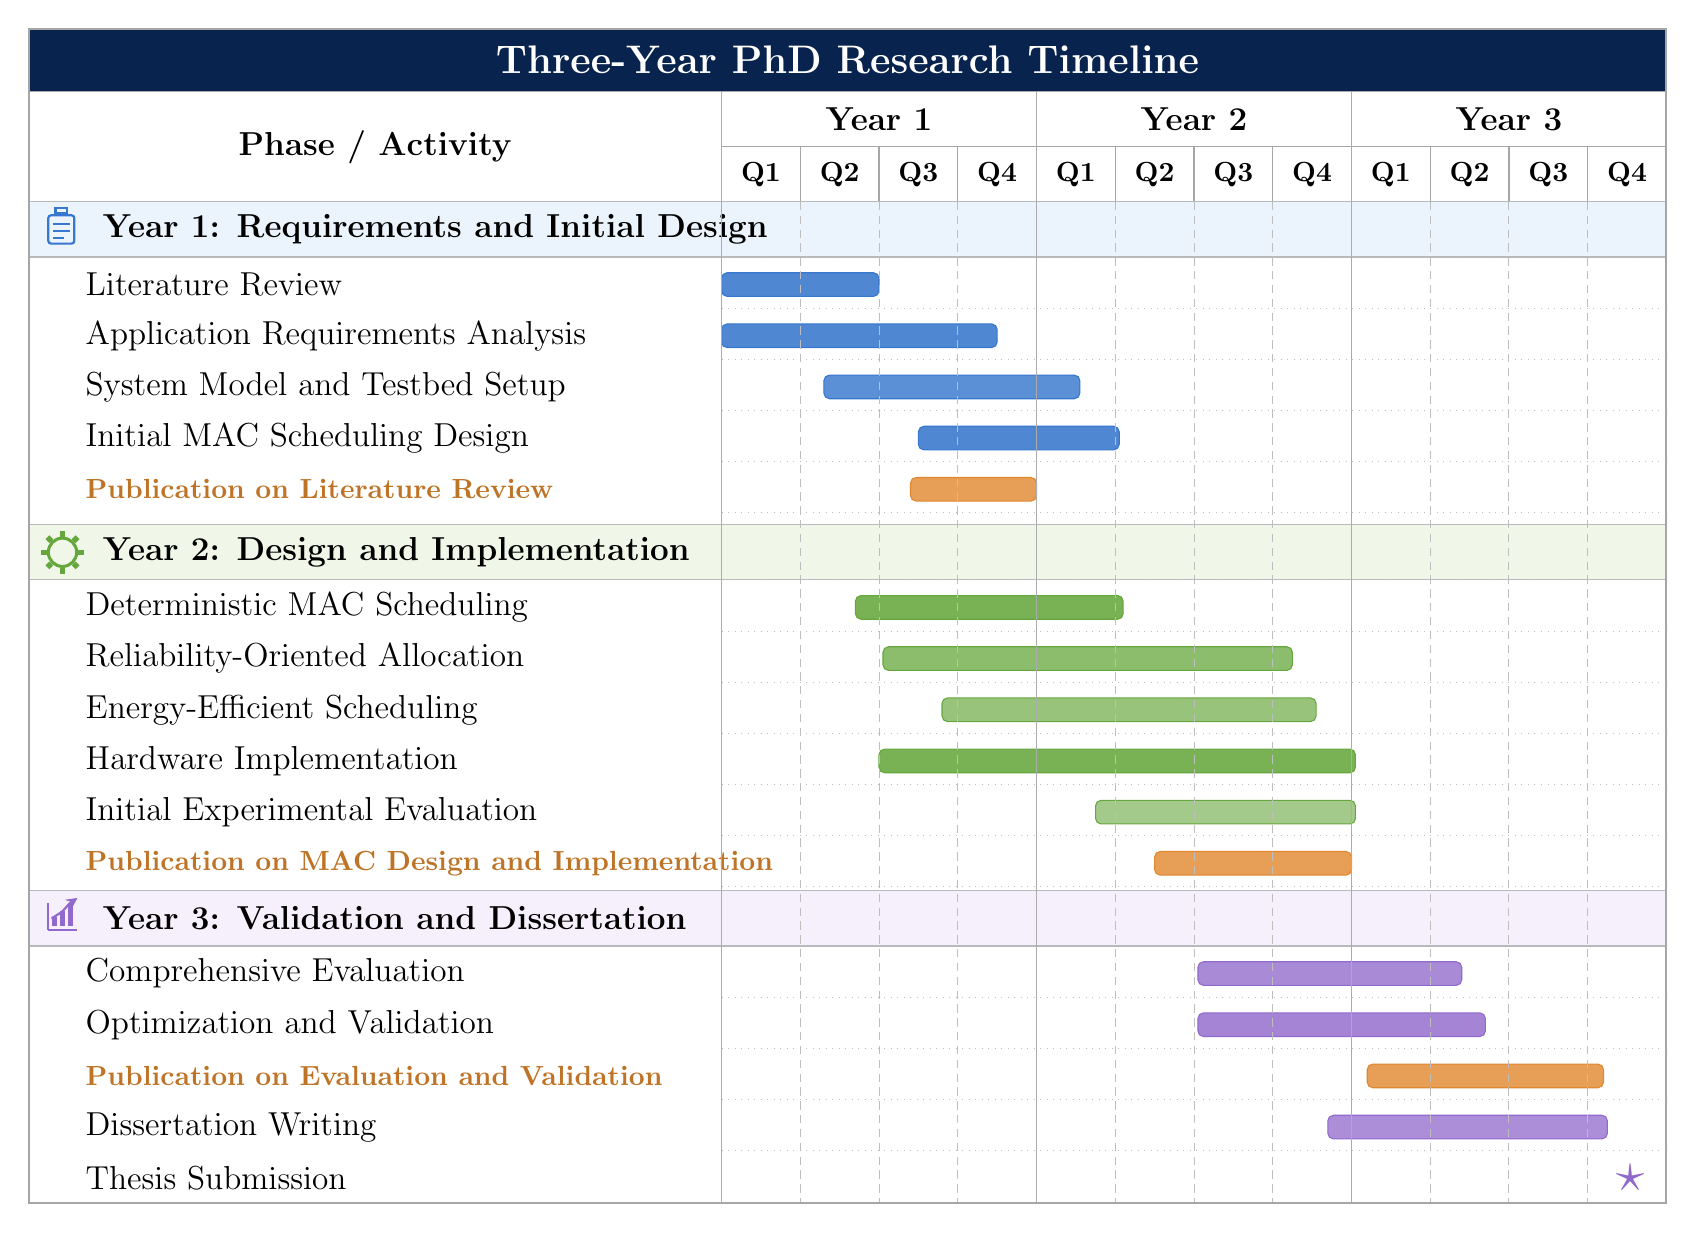
\begin{tikzpicture}[
    x=1cm,
    y=1cm,
    font=\small,
    task/.style={
        rounded corners=2pt,
        minimum height=0.28cm,
        inner sep=0pt
    }
]

% -------------------------------------------------
% Dimensions
% -------------------------------------------------
\def\labelwidth{8.8}
\def\quarterwidth{1.0}
\def\chartwidth{20.8}

% -------------------------------------------------
% Colors
% -------------------------------------------------
\definecolor{headerblue}{RGB}{8,35,78}
\definecolor{timelineblue}{RGB}{55,119,205}
\definecolor{timelinegreen}{RGB}{102,167,61}
\definecolor{timelinepurple}{RGB}{145,105,204}
\definecolor{timelineorange}{RGB}{225,135,45}

\definecolor{phaseblue}{RGB}{235,243,252}
\definecolor{phasegreen}{RGB}{240,247,233}
\definecolor{phasepurple}{RGB}{246,240,252}

\definecolor{gridgray}{RGB}{190,190,190}

% =================================================
% MAIN TITLE
% =================================================
\fill[headerblue] (0,0) rectangle (\chartwidth,-0.8);
\draw[gray!70] (0,0) rectangle (\chartwidth,-0.8);

\node[
    text=white,
    font=\bfseries\Large
] at (\chartwidth/2,-0.4)
{Three-Year PhD Research Timeline};

% =================================================
% LEFT HEADER: PHASE / ACTIVITY
% =================================================
\fill[white] (0,-0.8) rectangle (\labelwidth,-2.2);
\draw[gray!70] (0,-0.8) rectangle (\labelwidth,-2.2);

\node[
    font=\bfseries\large
] at (\labelwidth/2,-1.5)
{Phase / Activity};

% =================================================
% YEAR HEADERS
% =================================================
\foreach \x/\year in {
    8.8/Year 1,
    12.8/Year 2,
    16.8/Year 3
}{
    \fill[white] (\x,-0.8) rectangle ++(4,-0.7);
    \draw[gray!70] (\x,-0.8) rectangle ++(4,-0.7);

    \node[
        font=\bfseries\large
    ] at (\x+2,-1.15)
    {\year};
}

% =================================================
% QUARTER HEADERS
% =================================================
\foreach \i/\quarter in {
    0/Q1,1/Q2,2/Q3,3/Q4,
    4/Q1,5/Q2,6/Q3,7/Q4,
    8/Q1,9/Q2,10/Q3,11/Q4
}{
    \pgfmathsetmacro{\qx}{\labelwidth+\i}

    \fill[white]
        (\qx,-1.5)
        rectangle
        ++(\quarterwidth,-0.7);

    \draw[gray!70]
        (\qx,-1.5)
        rectangle
        ++(\quarterwidth,-0.7);

    \node[
        font=\bfseries
    ] at (\qx+0.5,-1.85)
    {\quarter};
}

% =================================================
% PHASE 1 HEADER
% =================================================
\fill[phaseblue] (0,-2.2) rectangle (\chartwidth,-2.9);
\draw[gray!55] (0,-2.2) rectangle (\chartwidth,-2.9);

% Small clipboard-style icon
\draw[timelineblue, line width=0.8pt, rounded corners=1pt]
    (0.25,-2.73) rectangle (0.58,-2.37);
\draw[timelineblue, line width=0.8pt]
    (0.34,-2.34) rectangle (0.49,-2.28);
\draw[timelineblue, line width=0.6pt]
    (0.31,-2.48) -- (0.52,-2.48);
\draw[timelineblue, line width=0.6pt]
    (0.31,-2.57) -- (0.52,-2.57);
\draw[timelineblue, line width=0.6pt]
    (0.31,-2.66) -- (0.45,-2.66);

\node[
    anchor=west,
    font=\bfseries\large
] at (0.82,-2.55)
{Year 1: Requirements and Initial Design};

% =================================================
% YEAR 1 ACTIVITIES
% =================================================
\node[anchor=west, font=\large]
    at (0.60,-3.25)
    {Literature Review};

\node[anchor=west, font=\large]
    at (0.60,-3.90)
    {Application Requirements Analysis};

\node[anchor=west, font=\large]
    at (0.60,-4.55)
    {System Model and Testbed Setup};

\node[anchor=west, font=\large]
    at (0.60,-5.20)
    {Initial MAC Scheduling Design};

\node[
    anchor=west,
    font=\normalsize\bfseries,
    text=timelineorange!85!black
] at (0.60,-5.85)
{Publication on Literature Review};

% Year 1 bars
\filldraw[
    task,
    fill=timelineblue!88,
    draw=timelineblue
]
(\labelwidth,-3.40)
rectangle
(\labelwidth+2.0,-3.10);

\filldraw[
    task,
    fill=timelineblue!88,
    draw=timelineblue
]
(\labelwidth,-4.05)
rectangle
(\labelwidth+3.50,-3.75);

\filldraw[
    task,
    fill=timelineblue!82,
    draw=timelineblue
]
(\labelwidth+1.30,-4.70)
rectangle
(\labelwidth+4.55,-4.40);

\filldraw[
    task,
    fill=timelineblue!88,
    draw=timelineblue
]
(\labelwidth+2.50,-5.35)
rectangle
(\labelwidth+5.05,-5.05);

% Year 1 publication bar
\filldraw[
    task,
    fill=timelineorange!80,
    draw=timelineorange
]
(\labelwidth+2.40,-6.00)
rectangle
(\labelwidth+4.00,-5.70);

% =================================================
% PHASE 2 HEADER
% =================================================
\fill[phasegreen] (0,-6.30) rectangle (\chartwidth,-7.00);
\draw[gray!55] (0,-6.30) rectangle (\chartwidth,-7.00);

% Small gear-style icon
\draw[
    timelinegreen,
    line width=1.1pt
]
(0.43,-6.65) circle (0.18);

\foreach \angle in {0,45,...,315}{
    \draw[
        timelinegreen,
        line width=2pt
    ]
    ($(0.43,-6.65)+(\angle:0.20)$)
    --
    ($(0.43,-6.65)+(\angle:0.27)$);
}

\node[
    anchor=west,
    font=\bfseries\large
] at (0.82,-6.65)
{Year 2: Design and Implementation};

% =================================================
% YEAR 2 ACTIVITIES
% =================================================
\node[anchor=west, font=\large]
    at (0.60,-7.35)
    {Deterministic MAC Scheduling};

\node[anchor=west, font=\large]
    at (0.60,-8.00)
    {Reliability-Oriented Allocation};

\node[anchor=west, font=\large]
    at (0.60,-8.65)
    {Energy-Efficient Scheduling};

\node[anchor=west, font=\large]
    at (0.60,-9.30)
    {Hardware Implementation};

\node[anchor=west, font=\large]
    at (0.60,-9.95)
    {Initial Experimental Evaluation};

\node[
    anchor=west,
    font=\normalsize\bfseries,
    text=timelineorange!85!black
] at (0.60,-10.60)
{Publication on MAC Design and Implementation};

% Year 2 bars
\filldraw[
    task,
    fill=timelinegreen!88,
    draw=timelinegreen
]
(\labelwidth+1.70,-7.50)
rectangle
(\labelwidth+5.10,-7.20);

\filldraw[
    task,
    fill=timelinegreen!75,
    draw=timelinegreen
]
(\labelwidth+2.05,-8.15)
rectangle
(\labelwidth+7.25,-7.85);

\filldraw[
    task,
    fill=timelinegreen!68,
    draw=timelinegreen
]
(\labelwidth+2.80,-8.80)
rectangle
(\labelwidth+7.55,-8.50);

\filldraw[
    task,
    fill=timelinegreen!88,
    draw=timelinegreen
]
(\labelwidth+2.00,-9.45)
rectangle
(\labelwidth+8.05,-9.15);

\filldraw[
    task,
    fill=timelinegreen!60,
    draw=timelinegreen
]
(\labelwidth+4.75,-10.10)
rectangle
(\labelwidth+8.05,-9.80);

% Year 2 publication bar
\filldraw[
    task,
    fill=timelineorange!80,
    draw=timelineorange
]
(\labelwidth+5.50,-10.75)
rectangle
(\labelwidth+8.00,-10.45);

% =================================================
% PHASE 3 HEADER
% =================================================
\fill[phasepurple] (0,-10.95) rectangle (\chartwidth,-11.65);
\draw[gray!55] (0,-10.95) rectangle (\chartwidth,-11.65);

% Small chart icon
\draw[
    timelinepurple,
    line width=0.8pt
]
(0.25,-11.45) -- (0.25,-11.10);

\draw[
    timelinepurple,
    line width=0.8pt
]
(0.25,-11.45) -- (0.62,-11.45);

\fill[timelinepurple]
    (0.30,-11.40) rectangle (0.36,-11.28);

\fill[timelinepurple]
    (0.40,-11.40) rectangle (0.46,-11.20);

\fill[timelinepurple]
    (0.50,-11.40) rectangle (0.56,-11.10);

\draw[
    timelinepurple,
    line width=0.8pt,
    -stealth
]
(0.29,-11.30)
--
(0.42,-11.22)
--
(0.52,-11.11)
--
(0.62,-11.04);

\node[
    anchor=west,
    font=\bfseries\large
] at (0.82,-11.30)
{Year 3: Validation and Dissertation};

% =================================================
% YEAR 3 ACTIVITIES
% =================================================
\node[anchor=west, font=\large]
    at (0.60,-12.00)
    {Comprehensive Evaluation};

\node[anchor=west, font=\large]
    at (0.60,-12.65)
    {Optimization and Validation};

\node[
    anchor=west,
    font=\normalsize\bfseries,
    text=timelineorange!85!black
] at (0.60,-13.30)
{Publication on Evaluation and Validation};

\node[anchor=west, font=\large]
    at (0.60,-13.95)
    {Dissertation Writing};

\node[anchor=west, font=\large]
    at (0.60,-14.60)
    {Thesis Submission};

% Year 3 bars
\filldraw[
    task,
    fill=timelinepurple!78,
    draw=timelinepurple
]
(\labelwidth+6.05,-12.15)
rectangle
(\labelwidth+9.40,-11.85);

\filldraw[
    task,
    fill=timelinepurple!82,
    draw=timelinepurple
]
(\labelwidth+6.05,-12.80)
rectangle
(\labelwidth+9.70,-12.50);

% Year 3 publication bar
\filldraw[
    task,
    fill=timelineorange!80,
    draw=timelineorange
]
(\labelwidth+8.20,-13.45)
rectangle
(\labelwidth+11.20,-13.15);

\filldraw[
    task,
    fill=timelinepurple!76,
    draw=timelinepurple
]
(\labelwidth+7.70,-14.10)
rectangle
(\labelwidth+11.25,-13.80);

% Thesis-submission milestone
\node[
    text=timelinepurple,
    font=\fontsize{22}{22}\selectfont
] at (\labelwidth+11.55,-14.60)
{$\star$};

% =================================================
% GRID AND OUTER BORDER
% =================================================

% Vertical divider after activity names
\draw[gray!65]
    (\labelwidth,-0.8)
    --
    (\labelwidth,-14.92);

% Dotted quarter grid
\foreach \i in {1,...,11}{
    \pgfmathsetmacro{\gx}{\labelwidth+\i}

    \draw[
        gridgray,
        densely dashed,
        line width=0.35pt
    ]
    (\gx,-2.2)
    --
    (\gx,-14.92);
}

% Strong year separators
\draw[gray!65, line width=0.7pt]
    (\labelwidth+4,-0.8)
    --
    (\labelwidth+4,-14.92);

\draw[gray!65, line width=0.7pt]
    (\labelwidth+8,-0.8)
    --
    (\labelwidth+8,-14.92);

% Horizontal task guides
\foreach \y in {
    -2.90,-3.55,-4.20,-4.85,-5.50,-6.15,
    -7.00,-7.65,-8.30,-8.95,-9.60,-10.25,-10.90,
    -11.65,-12.30,-12.95,-13.60,-14.25,-14.92
}{
    \draw[
        gridgray,
        dotted,
        line width=0.35pt
    ]
    (\labelwidth,\y)
    --
    (\chartwidth,\y);
}

% Outer frame
\draw[
    gray!70,
    line width=0.7pt
]
(0,0)
rectangle
(\chartwidth,-14.92);

\end{tikzpicture}%
}

\caption{Three-year timeline for the design, implementation, validation,
and dissemination of adaptive \gls{mac} scheduling and resource allocation
for DECT-2020 NR industrial \gls{iiot} networks.}
\label{fig:research-timeline}

\end{figure}
% =====================================================


\section{Expected Contributions}

The expected contributions of this research are both scientific and practical, addressing key challenges in \gls{nr} systems for industrial wireless communication.

\begin{itemize}

\item \textbf{Comprehensive Analysis of Scheduling Behavior}  
A detailed investigation of \gls{mac}-layer scheduling and its impact on system performance in \gls{nr}, including the interaction with hardware constraints and traffic dynamics.

\item \textbf{Measurement-Driven Characterization of Latency Components}  
A systematic decomposition of end-to-end latency into scheduling delay, transmission delay, and hardware-induced effects such as \gls{rx}-to-\gls{tx} turnaround time, based on real testbed measurements.

\item \textbf{Design of Adaptive Scheduling Mechanisms}  
Development of efficient and adaptive scheduling and resource allocation strategies tailored to the specific characteristics of \gls{nr} and industrial \gls{iiot} applications.

\item \textbf{Experimental Validation on Real DECT Testbed}  
Implementation and validation of the proposed approaches using a real \gls{nr} platform, providing practical insights beyond simulation-based studies.

\item \textbf{Performance Evaluation Framework}  
Establishment of a reproducible experimental framework for evaluating scheduling strategies in \gls{nr}, including standardized metrics such as \gls{thr}, \gls{lat}, \gls{jit}, and \gls{plr}.

\item \textbf{Design Guidelines for Industrial Deployments}  
Derivation of practical guidelines for designing efficient \gls{nr} systems in industrial environments, considering both protocol-level and hardware-level constraints.

\end{itemize}
\section{Publication Plan}

\begin{itemize}
    \item Paper 1: Measurement-Driven Latency Analysis of Uplink/Downlink Scheduling in DECT-2020 NR
    \item Paper 2: Experimental Performance Evaluation of a Multi-Vendor Private 5G Network
    \item Paper 3: DECT-2020 NR+: Architecture, MAC Design, Performance Evaluation, and Research Directions -- A Systematic Literature Review
    \item Paper 4: Experimental Evaluation of MAC Scheduling Strategies in DECT-2020 NR Testbeds
    \item Paper 5: Traffic-Aware Resource Allocation in DECT-2020 NR for Industrial IoT Applications
    \item Paper 6: Joint MAC Scheduling( Resource Allocation, Random Access) for Group assignment Scheduler for DECT-2020 NR Industrial Networks
    \item  Group-Based Scheduling and Resource Assignment for Scalable DECT-2020 NR Networks
\end{itemize}


\section{Conclusion}

This proposal presented a research plan focused on scheduling and resource allocation in  \gls{nr} networks for industrial wireless communication. With the increasing demand for reliable, low-latency, and scalable connectivity in \gls{iiot} environments, \gls{nr} has emerged as a promising technology due to its operation in license-exempt spectrum and its suitability for private deployments.

The analysis of existing literature and recent experimental studies indicates that, while \gls{nr} demonstrates strong potential in achieving low-latency communication, key challenges remain in the design of efficient \gls{mac}-layer scheduling and resource allocation mechanisms. In particular, practical system constraints such as \gls{tdd} operation and \gls{rx}-to-\gls{tx} turnaround significantly influence system performance and must be considered in scheduling design.

To address these challenges, this research proposes a measurement-driven and system-oriented approach that combines analytical modeling, experimental evaluation, and implementation on a real \gls{nr} platform. The work aims to develop adaptive scheduling and resource allocation strategies that improve throughput, latency, and reliability under realistic industrial traffic conditions.

The expected contributions include a comprehensive understanding of scheduling-performance trade-offs, the design of efficient \gls{mac}-layer mechanisms tailored to \gls{nr}, and the development of practical guidelines for industrial deployments. By bridging the gap between theoretical design and real-world implementation, this research is expected to contribute to the advancement of DECT-2020 \gls{nr} as a viable solution for next-generation industrial wireless systems.





\bibliographystyle{IEEEtran}
%\bibliography{references}
\bibliography{PHDDect}

\end{document}